% sample: clutter rate=50, best no. 014, worse no. 016

The second test scenario contains six independent objects that are born and die at different times. We have already discussed the influence of changing values over various parameters and will not include all the plots here, since every metric shows the exact same trend for all parameter values except for higher magnitudes of errors due to the increased number of objects. The reader can, however, find all figures in Appendix \ref{appendix:results-figures}. In this section, we will, however, compare two cases of trajectory estimation to point out the track continuity problem of the chosen tagging strategy.

First of all, let us examine the results of target state estimation of one sample, a worst-case scenario. In Figure \ref{fig:c2-results-overview}, we see how tracks, measurements, and clutter are generated along with state estimates depicted for two axes on the right side of the figure. We clearly see that for this exact sample there are many "holes" where the estimates were not suggested by the filter. One of the reasons for this behavior is false positive measurements that appear in close proximity to the real targets, which causes the filter to underestimate the likelihood of hypotheses of real target-to-measurement assignments.

\begin{figure*}
    \centering
    \begin{subfigure}[]{0.48\linewidth}
        \centering
        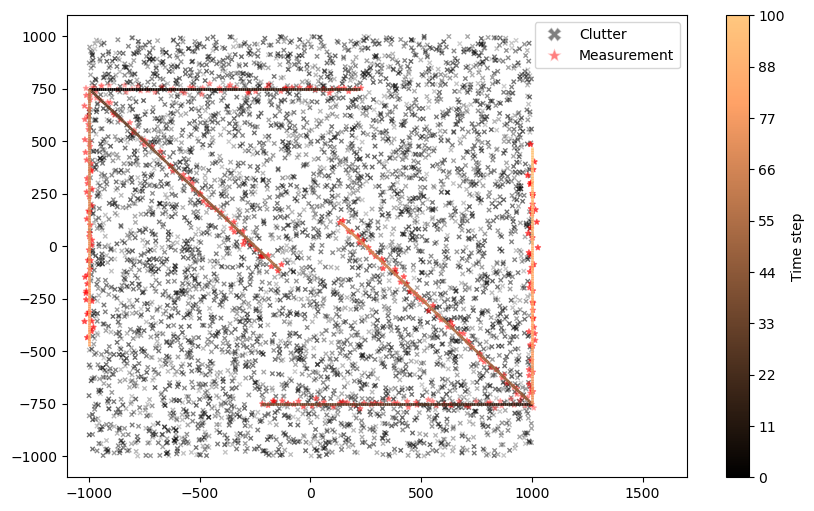
\includegraphics[width=\linewidth]{figures/c2-tracks-measurements.png}
    \end{subfigure}
    \hfill
    \begin{subfigure}[]{0.48\linewidth}
        \centering
        \begin{subfigure}[t]{\linewidth}
            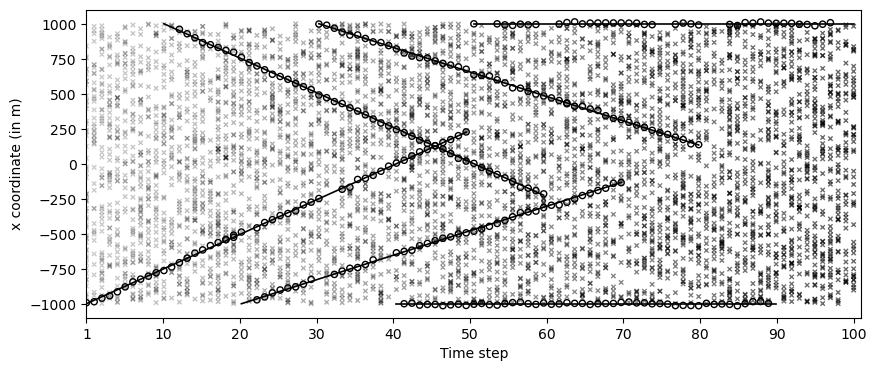
\includegraphics[width=\linewidth]{figures/c2-x-estimates.png}
        \end{subfigure}
        \vfill\par
        \begin{subfigure}[b]{\linewidth}
            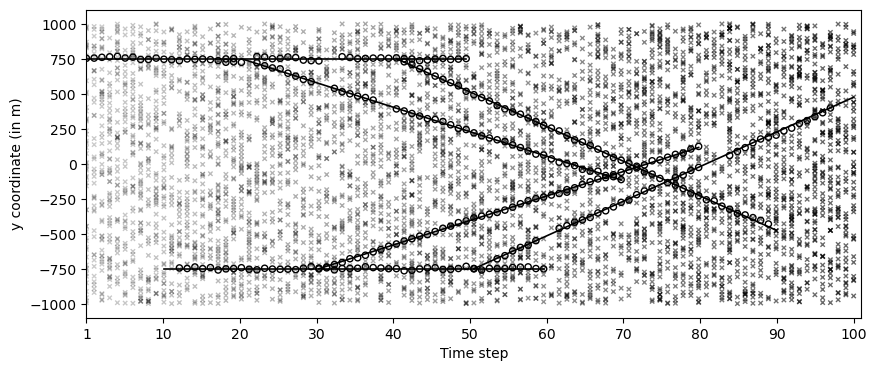
\includegraphics[width=\linewidth]{figures/c2-y-estimates.png}
        \end{subfigure}
    \end{subfigure}
  \caption[One sample of data and estimates for the (C2) scenario.]{One sample of data and estimates for the (C2) scenario. Left: True tracks of two objects (black to yellow) with clutter measurements (gray crosses) and received measurements (red stars) for a single Monte Carlo sample. Right: Change of both coordinates in time with noise measurements (red circles) and filter estimates (black circles) for the same Monte Carlo sample. In comparison to the (C1) scenario, the number of missed estimates is increased.}
  \label{fig:c2-results-overview}
\end{figure*}

The described behavior causes the track continuity problem already mentioned in the previous section. Figure \ref{fig:c2-track-continuity} compares two different runs on two different data samples. On the left picture, we see that there are six trajectory estimates for six targets, thus the estimate is correct. On the right image, however, the number of trajectories is higher, because tracks become terminated and new tracks are initialized. This is caused by the logic of tagging Gaussian components during merging. During this step of the GM-PHD filter, the component with the highest likelihood is chosen as the parent component, and other Gaussian terms are merged into the chosen one. If some new hypothesis created for a clutter measurement happens to have a higher weight, the Gaussian that had the initial tag is merged into this wrong component, and the correct tag disappears from the posterior intensity. The uncertainty in the posterior intensity is also shown in Figure \ref{fig:c2-post}. The best-case scenario is illustrated on the left. At time $k=100$, there is one target present in the scene, and the posterior intensity contains only one significant component. However, the bad scenario has a higher uncertainty in estimating the posterior PHD function, and we see several blobs in the image.

\begin{figure}
    \centering
    \begin{subfigure}[]{0.48\linewidth}
        \centering
        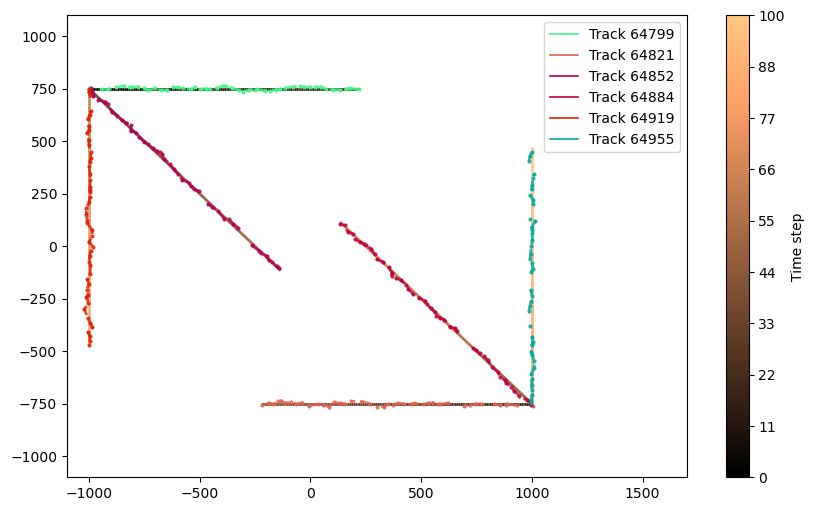
\includegraphics[width=\linewidth]{figures/c2-traj-good.png}
    \end{subfigure}
    \hfill
    \begin{subfigure}[]{0.48\linewidth}
        \centering
        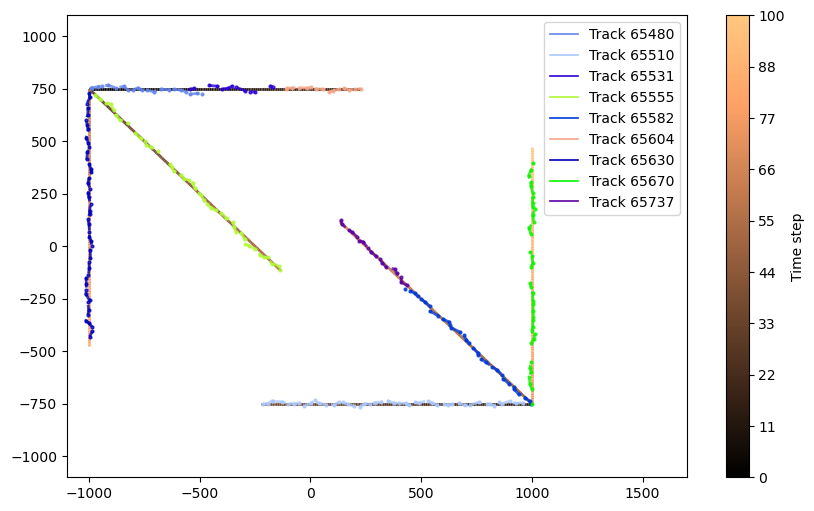
\includegraphics[width=\linewidth]{figures/c2-traj-bad.png}
    \end{subfigure}
  \caption[(C2). Comparison of trajectories estimates.]{Left: The visualization of trajectory estimates at time $k=100$ for the ideal case. For six targets, there are six different trajectories with good state estimates. Right: The same test scenario with wrong track estimates. We see that there are nine estimated trajectories, and the track continuity is not maintained. The filter was run with default settings, i.e., $\lambda_{c} = 12.5 \times 10^{-6}$, $P_{D,k} = 0.98$, $P_{S,k} = 0.99$, $\tau = 10^{-5}$, and $U=4$.}
  \label{fig:c2-track-continuity}
\end{figure}

\begin{figure}
    \centering
    \begin{subfigure}[]{0.48\linewidth}
        \centering
        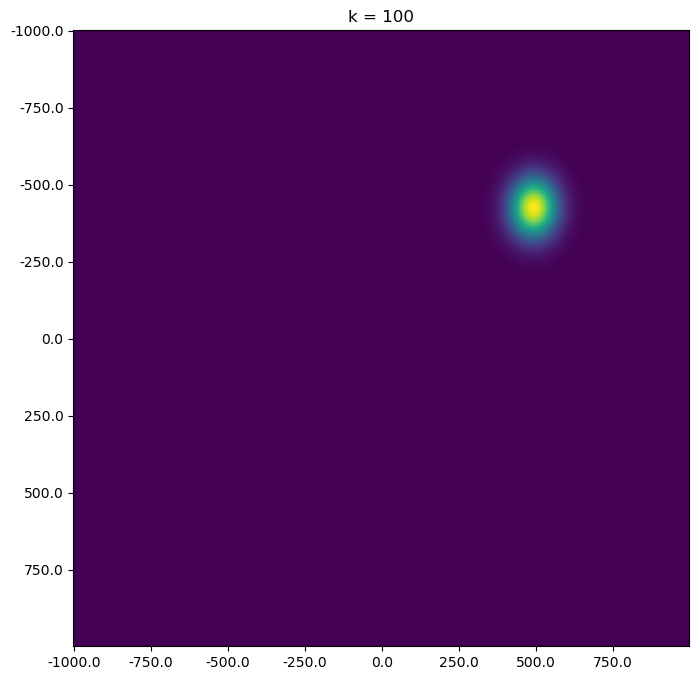
\includegraphics[width=\linewidth]{figures/c2-post-good.png}
    \end{subfigure}
    \hfill
    \begin{subfigure}[]{0.48\linewidth}
        \centering
        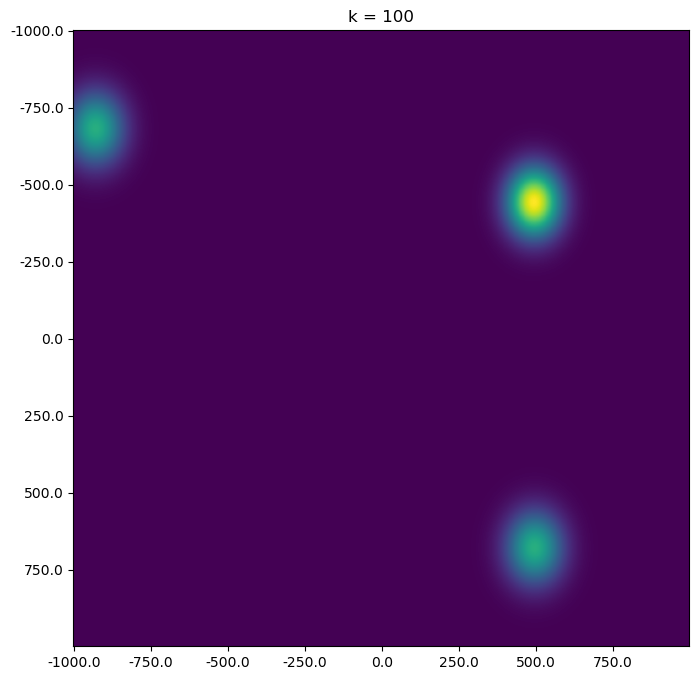
\includegraphics[width=\linewidth]{figures/c2-pos-bad.png}
    \end{subfigure}
  \caption[(C2). Comparison of posterior intensities for two cases.]{Left: The visualization of posterior intensity at time $k=100$. The intensity has only one Gaussian component with a high weight, which corresponds to the location of the only target present in the scene. Right: The posterior distribution at time step $k=100$ for a different sample of data. The uncertainty is higher, and there are three visible blobs for one existing target. Note that, for visualization purposes, the covariance matrices of all Gaussian components were multiplied by a factor of $81$. The filter was run with default settings, i.e. $\lambda_{c} = 12.5 \times 10^{-6}$, $P_{D,k} = 0.98$, $P_{S,k} = 0.99$, $\tau = 10^{-5}$, and $U=4$.}
  \label{fig:c2-post}
\end{figure}
